
\section{Gedämpfte Schwingungen}

\subsubsection{Dämpfung mit konstanter Reibungskraft}

\vspace{-0.2cm}

$$ m \ddot{x}(t) = -k x(t) - \mu F_N \quad \text{für } \ddot{x}(t) > 0 $$
$$ m \ddot{x}(t) = -k x(t) + \mu F_N \quad \text{für } \ddot{x}(t) < 0 $$

\smallskip

\begin{minipage}[c]{0.7\columnwidth}
    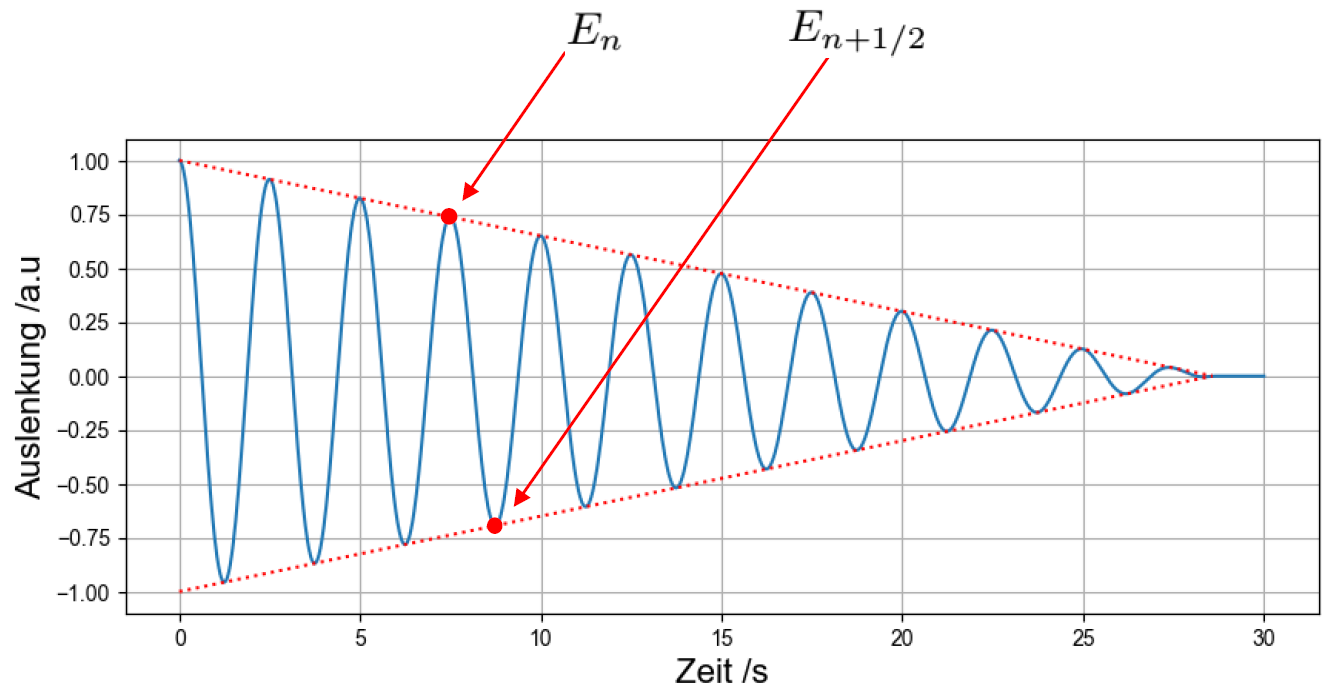
\includegraphics[width=\columnwidth]{images/gedaempfte_schwingungen_konst_reibung.png}
\end{minipage}
\hfill
\begin{minipage}[c]{0.28\columnwidth}
    $$ \boxed{ E = \frac{k \, A^2}{2} } $$
    $$ \boxed{ \Delta A = 4 \frac{F_R}{k}} $$
\end{minipage}


\begin{ctabular}{c l c}
    $E$         & Energie bei max. Auslenkung       & $[E] = \joule$                    \\
    $k=c$       & Federkonstante                    & $[k] = \frac{\newton}{\meter}$    \\
    $A$         & Amplitude bei max. Auslankung     & $[A] = \meter$                    \\
    $\Delta A$  & Amplitudenänderung pro Periode    & $[\Delta A] = \meter$             \\
    $F_R$       & Reibungskraft                     & $[F_R] = \newton$ 
\end{ctabular}


\subsection{Dämpfung proportional zur Geschwindigkeit}

\vspace{-0.2cm}
\[  
    \boxed{ \text{DGL:}  \quad \ddot{x}(t) + 2 \delta \, \dot{x}(t) + \omega^2 \, x(t) = 0 }
    \qquad \quad
    \boxed{ D = \frac{\delta}{\omega} = \frac{\kappa}{2 \omega} }
    \qquad \quad
    \boxed{ f = \frac{\Omega}{2 \, \pi} }
\]

\resizebox{\columnwidth}{!}{
    \begin{tabular}{lllll}
        \toprule
        Fall 1      & $\delta^2 - \omega^2 > 0$     & $D > 1$   & $x(t) = A e^{\lambda_1 t} + B e^{\lambda_2 t}$                            & Aperiodische Schwingung                                           \\
                    &                               &           &                                                                           & $\lambda_{1,2} = - \omega \left( D \pm \sqrt{D^2 -1} \right)$     \\
        \midrule    
        Fall 2      & $\delta^2 - \omega^2 < 0$     & $D < 1$   & $x(t) = A e^{- \delta t} \cdot \cos \left( \Omega t + \varphi \right)$    & Period. Schwingung (gedämpft)                                           \\
                    &                               &           &                                                                           & $\Omega^2 = \omega^2 \left( 1 - D^2 \right)$                      \\
        \midrule
        Fall 3      & $\delta^2 - \omega^2 = 0$     & $D = 1$   & $x(t) = (A + Bt) e^{- \delta t}$                                          & Grenzfall                                                         \\
        \bottomrule
    \end{tabular}
}

\medskip

\[
    \boxed{ \Omega^2 = \omega^2 - \delta^2  = \omega^2 - \left(\frac{\kappa}{2} \right)^2 }
    \qquad
    \boxed{ z \cdot \Lambda = \ln \left( \frac{A_n}{A_{n+z}} \right) = z \cdot \delta T = z \cdot \frac{\kappa}{2} T }
\]

\begin{ctabular}{c l c}
    $\delta = \frac{\kappa}{2}$ & Abklingkonstante                          & $[\kappa = \delta] = \frac{1}{\second}$ \\
    $\omega$                    & Kreisfrequenz ungedämpfte Schwingung      & $[\omega] = \frac{\rad}{\second}$ \\
    $D$                         & Dämpfungsgrad                             & $[D] = 1$ \\
    $\Omega$                    & Kreisfrequenz gedämpfte Schwingung        & $[\Omega] = \frac{\rad}{\second}$ \\
    $\Lambda$                   & Logarithmisches Dekrement                 & $[\Lambda] = 1$ \\
    $A_n$                       & Amplitude zum Zeitpunkt $t$               & $[A_n] = \meter$ \\
    $A_{n+z}$                   & Amplitude zum Zeitpunkt $t + z \cdot T$   & $[A_{n+z}] = \meter$ \\
    $z$                         & Anzahl verstrichene Schwingungen          & $[z] = 1$ \\
    $T$                         & Periodendauer                             & $[T] = \second$ \\
    $f$                         & Frequenz der gedämpften Schwingung        & $[f] = \hertz$ 
\end{ctabular}

